\chapter{Stops}
The Turing-Welchman Bombe was remarkably adept at computing daily
keys in a tractable manner. In optimal conditions,
with a well-crafted and fortunate menu, the Bombe could run in as
little as 20 minutes and produce exactly the daily key needed to
decrypt messages.
To approach these optimal conditions, we must consider what it means
for one menu to be stronger than another. In this chapter, we will
explore the relationship
between menus and the number of stops the Bombe is expected to
encounter. Equipped with this information, a cryptanalyst would be
able to select the menu
that yields the fewest stops. Each stop consumed precious
time as operators needed to verify whether they corresponded to a
valid key. Therefore, menu selection becomes an integral factor
in reducing the time between intercepting transmissions and
recovering the key for that day. Even a reduction of minutes could
provide the slight edge that the Allies needed to preempt an attack.
Thus, developing an accurate model by which we can correlate menus to
their expected number of stops is a matter of strategic urgency.

\section{Turing's Model}
We begin by describing the model for the expected number of stops given by Turing himself in the Prof's Book. Turing approaches this problem not by computing the expected number of stops itself, but instead by computing the expected number of {\bf{normal stops}} over all steckering hypothesis. These normal stops are described by Turing as ``positions at which by altering the point at which the current enters the diagonal board, one can make 25 relays close.'' In the case of a single loop in our menu, this is equivalent to the statement that the resulting loop in the Bombe has a singleton cycle. If we apply current to this singleton cycle all the remaining relays will close. For now we will ignore the impact of the diagonal board.
\\\\Turing considered a menu in which no loops occured which he called a {\bf{web}}. In this case every position of the Bombe and every initial steckering hypothesis would create a normal stop as there is no feedback necessary to electrify any additional wires on a given cable. Turing considers not only the $26^3$ possible rotor positions of the Bombe, but also the $26$ initial steckering hypotheses we could input. In our case, all steckering hypotheses and all rotor configurations produce a normal stop so we get $26^4$ total normal stops over all steckering hypotheses. In our simplified model with only $4$ characters this may look as follows
\begin{center}
	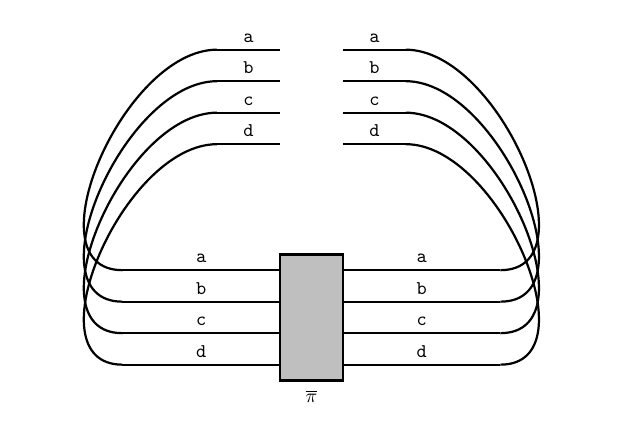
\begin{tikzpicture}[thick, scale=0.4, every node/.style={scale=0.7}]

		% Draw the wires entering the box
		\draw[-] (0, 2) -- (2, 2) node[midway, above] {\texttt{a}};
		\draw[-] (0, 1) -- (2, 1) node[midway, above] {\texttt{b}};
		\draw[-] (0, 0) -- (2, 0) node[midway, above] {\texttt{c}};
		\draw[-] (0,-1) -- (2,-1) node[midway, above] {\texttt{d}};

		% Draw the wires exiting the box with crossed mappings
		\draw[-] (4, 2) -- (6,2) node[midway, above] {\texttt{a}};
		\draw[-] (4, 1) -- (6, 1) node[midway, above] {\texttt{b}};
		\draw[-] (4, 0) -- (6, 0) node[midway, above] {\texttt{c}};
		\draw[-] (4,-1) -- (6, -1) node[midway, above] {\texttt{d}};

		\draw[-] (0-3, 2-7) to[out=180, in=180] (0, 2) node[midway, above] {};
		\draw[-] (0-3, 1-7) to[out=180, in=180] (0, 1) node[midway, above] {};
		\draw[-] (0-3, 0-7) to[out=180, in=180] (0, 0) node[midway, above] {};
		\draw[-] (0-3, -1-7) to[out=180, in=180] (0, -1)
		node[midway, above] {};

		\draw[-] (6+3, 2-7) to[out=360, in=360] (6, 2) node[midway, above] {};
		\draw[-] (6+3, 1-7) to[out=360, in=360] (6, 1) node[midway, above] {};
		\draw[-] (6+3, 0-7) to[out=360, in=360] (6, 0) node[midway, above] {};
		\draw[-] (6+3, -1-7) to[out=360, in=360] (6, -1)
		node[midway, above] {};

		% Draw the wires entering the box
		\draw[-] (0-3, 2-7) -- (2, 2-7) node[midway, above] {\texttt{a}};
		\draw[-] (0-3, 1-7) -- (2, 1-7) node[midway, above] {\texttt{b}};
		\draw[-] (0-3, 0-7) -- (2, 0-7) node[midway, above] {\texttt{c}};
		\draw[-] (0-3,-1-7) -- (2,-1-7) node[midway, above] {\texttt{d}};

		% Draw the wires exiting the box
		\draw[-] (2+2, 2-7) -- (4+5, 2-7) node[midway, above] {\texttt{a}};
		\draw[-] (2+2, 1-7) -- (4+5, 1-7) node[midway, above] {\texttt{b}};
		\draw[-] (2+2, 0-7) -- (4+5, 0-7) node[midway, above] {\texttt{c}};
		\draw[-] (2+2,-1-7) -- (4+5,-1-7) node[midway, above] {\texttt{d}};

		% Draw the lines inside the box to represent the mapping
		\draw[fill=lightgray] (2,-1.5-7) rectangle (4,2.5-7) node[midway] {};

		\node at (3, -2-7) {$\overline\pi$};


	\end{tikzpicture}
\end{center}
\noindent Turing then considered the effect of adding an edge to our menu which would have the effect of forming a loop, he called such an edge a {\bf{chain-closing constatation}}. He wanted to deduce the likelihood that adding such an edge turns our normal stops into anything other than a normal stop. We will denote this chain-closing edge as $s$. Our diagram would then be
\begin{center}
	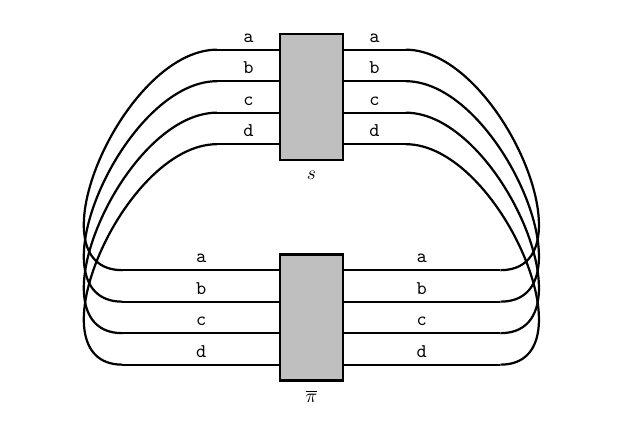
\begin{tikzpicture}[thick, scale=0.4, every node/.style={scale=0.7}]

		% Draw the lines inside the box to represent the mapping
		\draw[fill=lightgray] (2,-1.5) rectangle (4,2.5) node[midway] {};

		\node at (3, -2) {$s$};

		% Draw the wires entering the box
		\draw[-] (0, 2) -- (2, 2) node[midway, above] {\texttt{a}};
		\draw[-] (0, 1) -- (2, 1) node[midway, above] {\texttt{b}};
		\draw[-] (0, 0) -- (2, 0) node[midway, above] {\texttt{c}};
		\draw[-] (0,-1) -- (2,-1) node[midway, above] {\texttt{d}};

		% Draw the wires exiting the box with crossed mappings
		\draw[-] (4, 2) -- (6,2) node[midway, above] {\texttt{a}};
		\draw[-] (4, 1) -- (6, 1) node[midway, above] {\texttt{b}};
		\draw[-] (4, 0) -- (6, 0) node[midway, above] {\texttt{c}};
		\draw[-] (4,-1) -- (6, -1) node[midway, above] {\texttt{d}};

		\draw[-] (0-3, 2-7) to[out=180, in=180] (0, 2) node[midway, above] {};
		\draw[-] (0-3, 1-7) to[out=180, in=180] (0, 1) node[midway, above] {};
		\draw[-] (0-3, 0-7) to[out=180, in=180] (0, 0) node[midway, above] {};
		\draw[-] (0-3, -1-7) to[out=180, in=180] (0, -1)
		node[midway, above] {};

		\draw[-] (6+3, 2-7) to[out=360, in=360] (6, 2) node[midway, above] {};
		\draw[-] (6+3, 1-7) to[out=360, in=360] (6, 1) node[midway, above] {};
		\draw[-] (6+3, 0-7) to[out=360, in=360] (6, 0) node[midway, above] {};
		\draw[-] (6+3, -1-7) to[out=360, in=360] (6, -1)
		node[midway, above] {};

		% Draw the wires entering the box
		\draw[-] (0-3, 2-7) -- (2, 2-7) node[midway, above] {\texttt{a}};
		\draw[-] (0-3, 1-7) -- (2, 1-7) node[midway, above] {\texttt{b}};
		\draw[-] (0-3, 0-7) -- (2, 0-7) node[midway, above] {\texttt{c}};
		\draw[-] (0-3,-1-7) -- (2,-1-7) node[midway, above] {\texttt{d}};

		% Draw the wires exiting the box
		\draw[-] (2+2, 2-7) -- (4+5, 2-7) node[midway, above] {\texttt{a}};
		\draw[-] (2+2, 1-7) -- (4+5, 1-7) node[midway, above] {\texttt{b}};
		\draw[-] (2+2, 0-7) -- (4+5, 0-7) node[midway, above] {\texttt{c}};
		\draw[-] (2+2,-1-7) -- (4+5,-1-7) node[midway, above] {\texttt{d}};

		% Draw the lines inside the box to represent the mapping
		\draw[fill=lightgray] (2,-1.5-7) rectangle (4,2.5-7) node[midway] {};

		\node at (3, -2-7) {$\overline\pi$};


	\end{tikzpicture}
\end{center}
\noindent Suppose for a particular steckering hypothesis $S(x) = y$, the electrification of our hypothesis wire produces a normal stop. What is the probability that by adding the permutation $s$ we are now no longer in the situation of a normal stop?
\\\\Given that by supposition electrifying wire $xy$ through $\overline\pi$ has only a single live wire, the permutation $s$ need only connect the live wire to any of the $3$ remaining non-electrified wires to arrive at anything other than a normal stop. Thus there is $\frac{3}{4}$ chance that $s\circ\overline\pi$ is no longer a normal stop. Conversely, there is a $\frac{1}{4}$ chance that $s$ fails to remove our normal stop.
\\\\In the case of a $26$ character alphabet the same logic follows and we have a $\frac{1}{26}$ chance that a chain-closing constatations fails to remove a normal stop. Given that we originally expected $26^4$ normal stops over all steckering hypotheses without any closures, we would now expect that adding a chain-closing constatation to our menu would have $\frac{1}{26}$ as many normal stops. Thus adding one closure to our menu now brings the expected number of normal stops over all steckering hypotheses down to $26^{4-1} = 26^3$.
\\\\Turing extends this argument to explain that for a menu with $c$ loops (which he called {\bf{closures}}) we would expect $26^{4-c}$ normal stops over all steckering hypotheses.
\subsection{Dixon's Theorem}
A natural question arises - why should the number of normal stops over all steckering hypotheses approximate the number of stops? First, we are only considering a subset of possible stops so we might expect our approximation to be poor. Second, we are considering these stops over all steckering hypotheses so we might expect our approximation to be around $26$ times greater than the actual answer. Yet, testing Turing's formula against the actual Bombe, in many cases we find that his approximation of $26^{4-c}$ falls roughly in line with the actual number of stops. To answer this question we must show the following
\begin{enumerate}[(I)]
	\item The number of normal stops approximates the number of stops
	\item The consideration of all $26$ steckering hypotheses for each rotor position averages out in such a way that we get only $1$ steckering hypothesis per each rotor position thus removing any double counting of a particular rotor position.
\end{enumerate}
\subsubsection{Transitive Subgroups}
\noindent To show these two points, we require additional mathematical tools. We first need to translate our mechanical understanding of the Bombe's electrifcation of wires into a mathematical one. For a single loop this is quite trivial. If the permutation representing our loop is $\overline\pi$, then the number of normal stops over all steckering hypotheses is just the number of singleton cycles in $\overline\pi$'s cycle decomposition.
\\\\Once we add in additional closures this becomes slightly more complicated. Suppose we have two closures, with each seperate closure being represented by the permutations $\overline\pi$ and $\overline\delta$ respectively.
\begin{figure}[H]
	\begin{center}
		\scalebox{0.8}{
			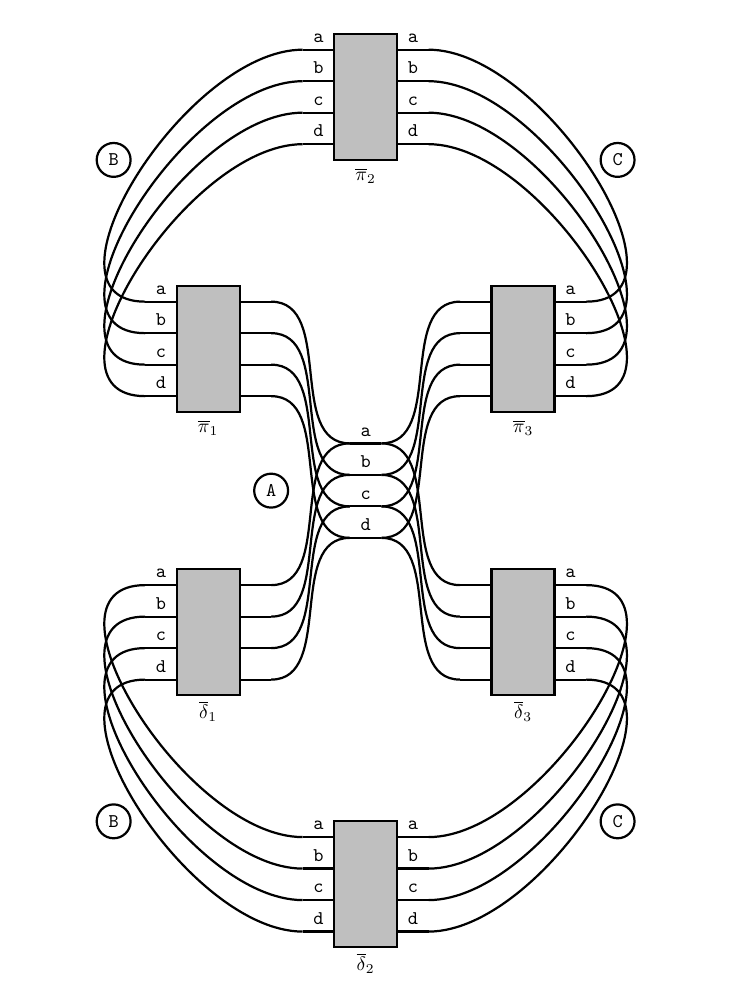
\begin{tikzpicture}[thick, scale=0.4, every node/.style={scale=0.7}]
				% Draw the box
				\draw[fill=lightgray] (0+5, 0+2) rectangle (2+5,4+2) node[midway] {};
				\node at (0+5+1, 0+2-0.5) {$\overline\pi_3$};

				% Draw the wires exiting the box
				\draw[-] (7, 5.5) -- (8,5.5) node[midway, above] {\texttt{a}};
				\draw[-] (7, 4.5) -- (8,4.5) node[midway, above] {\texttt{b}};
				\draw[-] (7, 3.5) -- (8, 3.5) node[midway, above] {\texttt{c}};
				\draw[-] (7,2.5) -- (8, 2.5) node[midway, above] {\texttt{d}};

				% Draw the wires entering the box
				\draw[-] (4, 5.5) -- (5,5.5) node[midway, above] {};
				\draw[-] (4, 4.5) -- (5,4.5) node[midway, above] {};
				\draw[-] (4, 3.5) -- (5, 3.5) node[midway, above] {};
				\draw[-] (4,2.5) -- (5, 2.5) node[midway, above] {};

				\draw[fill=lightgray] (0-5,0+2) rectangle (2-5,4+2) node[midway] {};
				\node at (0-5+1, 0+2-0.5) {$\overline\pi_1$};

				% Draw the wires entering the box
				\draw[-] (-13+7, 5.5) -- (-13+8,5.5) node[midway, above] {\texttt{a}};
				\draw[-] (-13+7, 4.5) -- (-13+8,4.5) node[midway, above] {\texttt{b}};
				\draw[-] (-13+7, 3.5) -- (-13+8, 3.5) node[midway, above] {\texttt{c}};
				\draw[-] (-13+7,2.5) -- (-13+8, 2.5) node[midway, above] {\texttt{d}};

				% Draw the wires exiting the box
				\draw[-] (-13+7+3, 5.5) -- (-13+8+3,5.5) node[midway, above] {};
				\draw[-] (-13+7+3, 4.5) -- (-13+8+3,4.5) node[midway, above] {};
				\draw[-] (-13+7+3, 3.5) -- (-13+8+3, 3.5) node[midway, above] {};
				\draw[-] (-13+7+3,2.5) -- (-13+8+3, 2.5) node[midway, above] {};

				\draw[fill=lightgray] (0,0+10) rectangle (2,4+10) node[midway] {};
				\node at (0+1, 0+10-0.5) {$\overline\pi_2$};

				% Draw the wires entering the box
				\draw[-] (-1, 3+10.5) -- (0, 3+10.5) node[midway, above] {\texttt{a}};
				\draw[-] (-1, 2+10.5) -- (0, 2+10.5) node[midway, above] {\texttt{b}};
				\draw[-] (-1, 1+10.5) -- (0, 1+10.5) node[midway, above] {\texttt{c}};
				\draw[-] (-1,0+10.5) -- (0,0+10.5) node[midway, above] {\texttt{d}};

				% Draw the wires exiting the box
				\draw[-] (3+-1, 3+10.5) -- (3+0, 3+10.5) node[midway, above]
				{\texttt{a}};
				\draw[-] (3+-1, 2+10.5) -- (3+0, 2+10.5) node[midway, above]
				{\texttt{b}};
				\draw[-] (3+-1, 1+10.5) -- (3+0, 1+10.5) node[midway, above]
				{\texttt{c}};
				\draw[-] (3+-1,0+10.5) -- (3+0,0+10.5) node[midway, above] {\texttt{d}};

				% Draw wires from 2 to 1
				\draw[-] (-6, 5.5) to[out=180, in=180] (-1, 13.5)
				node[midway, above] {};
				\draw[-] (-6, 4.5) to[out=180, in=180] (-1, 12.5)
				node[midway, above] {};
				\draw[-] (-6, 3.5) to[out=180, in=180] (-1, 11.5)
				node[midway, above] {};
				\draw[-] (-6, 2.5) to[out=180, in=180] (-1, 10.5)
				node[midway, above] {};

				% Draw wires from 3 to 2
				\draw[-] (8, 5.5) to[out=360, in=360] (3, 13.5) node[midway, above] {};
				\draw[-] (8, 4.5) to[out=360, in=360] (3, 12.5) node[midway, above] {};
				\draw[-] (8, 3.5) to[out=360, in=360] (3, 11.5) node[midway, above] {};
				\draw[-] (8, 2.5) to[out=360, in=360] (3, 10.5)
				node[midway, above] {};

				% Midway wires
				\draw[-] (0.5, 1) -- (1.5, 1) node[midway, above] {\texttt{a}};
				\draw[-] (0.5, 0) -- (1.5, 0) node[midway, above] {\texttt{b}};
				\draw[-] (0.5, -1) -- (1.5, -1) node[midway, above] {\texttt{c}};
				\draw[-] (0.5,-2) -- (1.5,-2) node[midway, above] {\texttt{d}};

				% Draw wires from 1 to midway
				\draw[-] (-2, 5.5) to[out=360, in=180] (0.5, 1) node[midway, above] {};
				\draw[-] (-2, 4.5) to[out=360, in=180] (0.5, 0) node[midway, above] {};
				\draw[-] (-2, 3.5) to[out=360, in=180] (0.5, -1) node[midway, above] {};
				\draw[-] (-2, 2.5) to[out=360, in=180] (0.5, -2) node[midway, above] {};

				% Draw wires from 2 to midway
				\draw[-] (4, 5.5) to[out=180, in=360] (1.5, 1) node[midway, above] {};
				\draw[-] (4, 4.5) to[out=180, in=360] (1.5, 0) node[midway, above] {};
				\draw[-] (4, 3.5) to[out=180, in=360] (1.5, -1) node[midway, above] {};
				\draw[-] (4, 2.5) to[out=180, in=360] (1.5, -2) node[midway, above] {};

				\draw[fill=lightgray] (0,0-15) rectangle (2,4-15) node[midway] {};
				\node at (0+1, 0+10-0.5-25) {$\overline\delta_2$};

				% Draw the wires entering the box
				\draw[-] (-1, 3+10.5-25) -- (0, 3+10.5-25) node[midway,
					above] {\texttt{a}};
				\draw[-] (-1, 2+10.5-25) -- (0, 2+10.5-25) node[midway,
					above] {\texttt{b}};
				\draw[-] (-1, 1+10.5-25) -- (0, 1+10.5-25) node[midway,
					above] {\texttt{c}};
				\draw[-] (-1,0+10.5-25) -- (0,0+10.5-25) node[midway, above]
				{\texttt{d}};

				% Draw the wires exiting the box
				\draw[-] (3+-1, 3+10.5-25) -- (3+0, 3+10.5-25) node[midway,
					above] {\texttt{a}};
				\draw[-] (3+-1, 2+10.5-25) -- (3+0, 2+10.5-25) node[midway,
					above] {\texttt{b}};
				\draw[-] (3+-1, 1+10.5-25) -- (3+0, 1+10.5-25) node[midway,
					above] {\texttt{c}};
				\draw[-] (3+-1,0+10.5-25) -- (3+0,0+10.5-25) node[midway,
					above] {\texttt{d}};

				\draw[fill=lightgray] (0-5,0+2-9) rectangle (2-5,4+2-9) node[midway] {};
				\node at (0-5+1, 0+2-0.5-9) {$\overline\delta_1$};

				% Draw the wires entering the box
				\draw[-] (-13+7, 5.5-9) -- (-13+8,5.5-9) node[midway, above]
				{\texttt{a}};
				\draw[-] (-13+7, 4.5-9) -- (-13+8,4.5-9) node[midway, above]
				{\texttt{b}};
				\draw[-] (-13+7, 3.5-9) -- (-13+8, 3.5-9) node[midway, above]
				{\texttt{c}};
				\draw[-] (-13+7,2.5-9) -- (-13+8, 2.5-9) node[midway, above]
				{\texttt{d}};

				% Draw the wires exiting the box
				\draw[-] (-13+7+3, 5.5-9) -- (-13+8+3,5.5-9) node[midway, above] {};
				\draw[-] (-13+7+3, 4.5-9) -- (-13+8+3,4.5-9) node[midway, above] {};
				\draw[-] (-13+7+3, 3.5-9) -- (-13+8+3, 3.5-9) node[midway, above] {};
				\draw[-] (-13+7+3,2.5-9) -- (-13+8+3, 2.5-9) node[midway, above] {};

				% Draw the box
				\draw[fill=lightgray] (0+5, 0+2-9) rectangle (2+5,4+2-9)
				node[midway] {};
				\node at (0+5+1, 0+2-0.5-9) {$\overline\delta_3$};

				% Draw the wires exiting the box
				\draw[-] (7, 5.5-9) -- (8,5.5-9) node[midway, above] {\texttt{a}};
				\draw[-] (7, 4.5-9) -- (8,4.5-9) node[midway, above] {\texttt{b}};
				\draw[-] (7, 3.5-9) -- (8, 3.5-9) node[midway, above] {\texttt{c}};
				\draw[-] (7,2.5-9) -- (8, 2.5-9) node[midway, above] {\texttt{d}};

				% Draw the wires entering the box
				\draw[-] (4, 5.5-9) -- (5,5.5-9) node[midway, above] {};
				\draw[-] (4, 4.5-9) -- (5,4.5-9) node[midway, above] {};
				\draw[-] (4, 3.5-9) -- (5, 3.5-9) node[midway, above] {};
				\draw[-] (4,2.5-9) -- (5, 2.5-9) node[midway, above] {};

				% Draw wires from 4 to 5
				\draw[-] (-6, 5.5-9) to[out=180, in=180] (-1, 13.5-25)
				node[midway, above] {};
				\draw[-] (-6, 4.5-9) to[out=180, in=180] (-1, 12.5-25)
				node[midway, above] {};
				\draw[-] (-6, 3.5-9) to[out=180, in=180] (-1, 11.5-25)
				node[midway, above] {};
				\draw[-] (-6, 2.5-9) to[out=180, in=180] (-1, 10.5-25)
				node[midway, above] {};

				% Draw wires from 5 to 6
				\draw[-] (8, 5.5-9) to[out=360, in=360] (3, 13.5-25)
				node[midway, above] {};
				\draw[-] (8, 4.5-9) to[out=360, in=360] (3, 12.5-25)
				node[midway, above] {};
				\draw[-] (8, 3.5-9) to[out=360, in=360] (3, 11.5-25)
				node[midway, above] {};
				\draw[-] (8, 2.5-9) to[out=360, in=360] (3, 10.5-25)
				node[midway, above] {};

				% Draw wires from 4 to midway
				\draw[-] (-2, 5.5-9) to[out=360, in=180] (0.5, 1)
				node[midway, above] {};
				\draw[-] (-2, 4.5-9) to[out=360, in=180] (0.5, 0)
				node[midway, above] {};
				\draw[-] (-2, 3.5-9) to[out=360, in=180] (0.5, -1)
				node[midway, above] {};
				\draw[-] (-2, 2.5-9) to[out=360, in=180] (0.5, -2)
				node[midway, above] {};

				% Draw wires from 2 to midway
				\draw[-] (4, 5.5-9) to[out=180, in=360] (1.5, 1) node[midway, above] {};
				\draw[-] (4, 4.5-9) to[out=180, in=360] (1.5, 0) node[midway, above] {};
				\draw[-] (4, 3.5-9) to[out=180, in=360] (1.5, -1)
				node[midway, above] {};
				\draw[-] (4, 2.5-9) to[out=180, in=360] (1.5, -2)
				node[midway, above] {};
				\node[draw,circle] at (-2, -0.5) {\texttt{A}};
				\node[draw,circle] at (-7, -11) {\texttt{B}};
				\node[draw,circle] at (-7, -11+21) {\texttt{B}};
				\node[draw,circle] at (-7+16, -11) {\texttt{C}};
				\node[draw,circle] at (-7+16, -11+21) {\texttt{C}};

			\end{tikzpicture}
		}
	\end{center}
\end{figure}
\noindent How can we determine which wires are connected to which in this complex arrangment of permutations? To answer this we introduce
\begin{definition}
	The subgroup of $S_n$ generated by two permutations $\sigma$, $\tau$ $\in S_n$ is
	\begin{center}
		$\langle\sigma,\tau\rangle \coloneq \{\sigma^{a_1}\tau^{b_1}\dots\sigma^{a_k}\tau^{b_k}\text{ }|\text{ }k\in\mathbb{N},\text{ }a_i,b_i\in\mathbb{Z}\}$
	\end{center}
\end{definition}
\noindent This is the set of all group elements obtained by applying finite compositions of $\sigma$, $\tau$, and their inverses.
\\\\Consider how this relates to our two loop Bombe arrangment with $\overline\pi$ and $\overline\delta$. The electricity is free to flow through any number of iterations forwards and backwards through both $\overline\pi$ and $\overline\delta$. Applying a current at some input wire will propogate in such a way that it reaches possible letters which can be reached by some sequence of applications of $\overline\pi$, $\overline\delta$, and their inverses. Then on cable \texttt{A}, applying a current at some input $x$ can only reach wire $y$ on that cable if $\exists\text{ }\sigma\in\langle\overline\pi, \overline\delta\rangle$ such that $\sigma(x) = y$. If we want to know for a given input wire, what other wires it can reach, we need to know which letters are connected to which through permutations in $\langle\overline\pi, \overline\delta\rangle$.
\\\\We note that $\langle\overline\pi, \overline\delta\rangle$ has a natural group action on $\mathbb{N}_{4}$ given by
\begin{align*}
	\sigma\cdot{x} \coloneq \sigma(x)\text{ for }\sigma\in\langle\overline\pi, \overline\delta\rangle\text{ and }x\in\mathbb{N}_{4}.
\end{align*}
Consider an orbit for this group action. That is, for $x\in\mathbb{N}_{4}$ we have
\begin{center}
	$\langle\overline\pi, \overline\delta\rangle\cdot x\coloneq\{\sigma(x)\text{ }|\text{ }\sigma\in\langle\overline\pi, \overline\delta\rangle\}$
\end{center}
\noindent We can think of this orbit as all elements in $\mathbb{N}_{4}$ which $x$ can reach via some sequence finite compositions of $\overline\pi$, $\overline\delta$, and their inverses. This is exactly analogous to the set of wires on cable \texttt{A} which can be reached from an input on $x$. Then these orbits partition $\mathbb{N}_{4}$ and tell us which wires are in a connected loop in our Bombe arrangement.
\\\\In this way the parition given by the set of orbits $\mathbb{N}_{4}/\langle\overline\pi, \overline\delta\rangle$ represents which wires are connected to which wires in our diagram. If $\mathbb{N}_{4}/\langle\overline\pi, \overline\delta\rangle = \{\{\texttt{a},\dots,\texttt{d}\}\}$ then we know that electrifying any wire on cable \texttt{A} will electrify all wires in the diagram. In such a case we say that $\langle\overline\pi, \overline\delta\rangle$ forms a {\bf{transitive subgroup}}.
\\\\Consider how this relates to our single loop example.
\begin{center}
	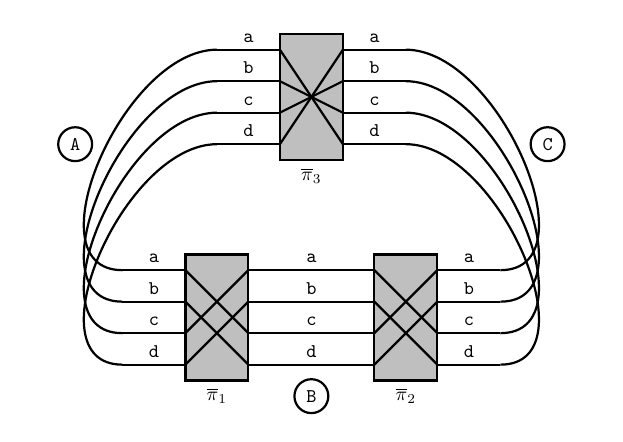
\begin{tikzpicture}[thick, scale=0.4, every node/.style={scale=0.7}]
		% Draw the box
		\draw[fill=lightgray] (2,-1.5) rectangle (4,2.5) node[midway] {};

		\node at (3, -2) {$\overline\pi_3$};

		% Draw the wires entering the box
		\draw[-] (0, 2) -- (2, 2) node[midway, above] {\texttt{a}};
		\draw[-] (0, 1) -- (2, 1) node[midway, above] {\texttt{b}};
		\draw[-] (0, 0) -- (2, 0) node[midway, above] {\texttt{c}};
		\draw[-] (0,-1) -- (2,-1) node[midway, above] {\texttt{d}};

		% Draw the wires exiting the box with crossed mappings
		\draw[-] (4, 2) -- (6,2) node[midway, above] {\texttt{a}};
		\draw[-] (4, 1) -- (6, 1) node[midway, above] {\texttt{b}};
		\draw[-] (4, 0) -- (6, 0) node[midway, above] {\texttt{c}};
		\draw[-] (4,-1) -- (6, -1) node[midway, above] {\texttt{d}};

		% Draw the lines inside the box to represent the mapping
		\draw[-] (2, 2) -- (4,-1);
		\draw[-] (2, 1) -- (4, 0);
		\draw[-] (2, 0) -- (4, 1);
		\draw[-] (2,-1) -- (4, 2);

		\draw[-] (0-3, 2-7) to[out=180, in=180] (0, 2) node[midway, above] {};
		\draw[-] (0-3, 1-7) to[out=180, in=180] (0, 1) node[midway, above] {};
		\draw[-] (0-3, 0-7) to[out=180, in=180] (0, 0) node[midway, above] {};
		\draw[-] (0-3, -1-7) to[out=180, in=180] (0, -1)
		node[midway, above] {};

		\draw[-] (6+3, 2-7) to[out=360, in=360] (6, 2) node[midway, above] {};
		\draw[-] (6+3, 1-7) to[out=360, in=360] (6, 1) node[midway, above] {};
		\draw[-] (6+3, 0-7) to[out=360, in=360] (6, 0) node[midway, above] {};
		\draw[-] (6+3, -1-7) to[out=360, in=360] (6, -1)
		node[midway, above] {};

		\draw[fill=lightgray] (2-3,-1.5-7) rectangle (4-3,2.5-7) node[midway] {};

		\node at (3-3, -2-7) {$\overline\pi_1$};

		% Draw the wires entering the box
		\draw[-] (0-3, 2-7) -- (2-3, 2-7) node[midway, above] {\texttt{a}};
		\draw[-] (0-3, 1-7) -- (2-3, 1-7) node[midway, above] {\texttt{b}};
		\draw[-] (0-3, 0-7) -- (2-3, 0-7) node[midway, above] {\texttt{c}};
		\draw[-] (0-3,-1-7) -- (2-3,-1-7) node[midway, above] {\texttt{d}};

		% Draw the wires exiting the box
		\draw[-] (4-3, 2-7) -- (6-3,2-7) node[right, above] {\texttt{a}};
		\draw[-] (4-3, 1-7) -- (6-3, 1-7) node[right, above] {\texttt{b}};
		\draw[-] (4-3, 0-7) -- (6-3, 0-7) node[right, above] {\texttt{c}};
		\draw[-] (4-3,-1-7) -- (6-3, -1-7) node[right, above] {\texttt{d}};

		% Draw the lines inside the box to represent the mapping
		\draw[-] (2-3, 2-7) -- (4-3, 0-7);
		\draw[-] (2-3, 1-7) -- (4-3, -1-7);
		\draw[-] (2-3, 0-7) -- (4-3, 2-7);
		\draw[-] (2-3,-1-7) -- (4-3, 1-7);

		\draw[fill=lightgray] (2+3,-1.5-7) rectangle (4+3,2.5-7) node[midway] {};

		\node at (3+3, -2-7) {$\overline\pi_2$};

		% Draw the wires entering the box
		\draw[-] (0+3, 2-7) -- (2+3, 2-7) node[midway, above] {};
		\draw[-] (0+3, 1-7) -- (2+3, 1-7) node[midway, above] {};
		\draw[-] (0+3, 0-7) -- (2+3, 0-7) node[midway, above] {};
		\draw[-] (0+3,-1-7) -- (2+3,-1-7) node[midway, above] {};

		% Draw the wires exiting the box
		\draw[-] (4+3, 2-7) -- (6+3,2-7) node[midway, above] {\texttt{a}};
		\draw[-] (4+3, 1-7) -- (6+3, 1-7) node[midway, above] {\texttt{b}};
		\draw[-] (4+3, 0-7) -- (6+3, 0-7) node[midway, above] {\texttt{c}};
		\draw[-] (4+3,-1-7) -- (6+3, -1-7) node[midway, above] {\texttt{d}};

		\draw[-] (2+3, 2-7) -- (4+3, 0-7);
		\draw[-] (2+3, 1-7) -- (4+3, -1-7);
		\draw[-] (2+3, 0-7) -- (4+3, 2-7);
		\draw[-] (2+3,-1-7) -- (4+3, 1-7);
		\node[draw,circle] at (-4.5, -1) {\texttt{A}};
		\node[draw,circle] at (3, -9) {\texttt{B}};
		\node[draw,circle] at (10.5, -1) {\texttt{C}};
	\end{tikzpicture}
\end{center}
\noindent In this loop, we have that on cable \texttt{A}, wires \texttt{a} and \texttt{d} are connected, and wires \texttt{b} and \texttt{c} are connected. We explained that his could be simply determined by examining the cycle decomposition of $\overline\pi$ which in this case is
\begin{center}
	(\texttt{ad})(\texttt{bc})
\end{center}
\noindent However, we can get the exact same picture by simply considering the set orbits of $\langle\overline\pi\rangle$ acting on $\{\texttt{a},\dots\texttt{z}\}$, which would give us
\begin{center}
	$\{\{\texttt{a}, \texttt{d}\},\{\texttt{b}, \texttt{c}\}\}$
\end{center}
\noindent which gives us an equal picture of the connections between wires on the \texttt{A} cable. Additionally, shifting to this view means that rather than saying the entire loop becomes electrified when $\overline\pi$ has a $26^1$ cycle type, we say that this occurs when $\langle\overline\pi\rangle$ forms a transitive subgroup of $S_4$.
\\\\This description is more robust in that it can handle any number of closures and gives us a picture of which wires are connected to which on a particular cable.
\subsubsection{Distribution of Stops}
Equipped with this mathematical framework are now ready to address Turing's model. We will classify stops by the cardinality and multiplicty of sets in the partition given by the orbits described above. For example, if a set of orbits is
\begin{center}
	$\{\{\texttt{a}, \dots, \texttt{m}\}, \{\texttt{n}, \dots, \texttt{z}\}\}$
\end{center}
we would say this stop is a $13^2$ stop. This is effectively analogous to the cycle type of a permutation but in order to extend this to multiple loops we must frame it in this description of partitions given by orbits of subgroups. We will call these orbit orbit structures.
\\\\In Turing's model, such a $13^2$ stop as above, would count as $0$ normal stops over all steckering hypotheses, In the actual running of the Bombe this would constitute a single stop. Further, a $1^323^1$ stop in Turing's model would be considered as $3$ normal stops over all possible steckering hypotheses. In reality this would only constitute a single real stop in the running of the Bombe. This highlights the two qualms that we are trying to reconcile in Turing's model, the absence of abnormal stops, and the overcounting of normal stops.
\\\\We begin by considering the case of $2$ closures, where at each rotor position of the Bombe, we have some permutations $\overline\pi$ and $\overline\delta$. What is the distribution of stop types? For now we will assume that any loop in a particular configuration of the Bombe represents a random permutation. We will later refine this, but as a heuristic it serves to justify Turing's model. We want to know what stop types are most common. That is, given two random permutations $\overline\pi$ and $\overline\delta$, what is the distribution of orbit structures for the subgroup $\langle\overline\pi, \overline\delta\rangle$? This question was answered by John Dixon in 1969 in his paper ``The Probability of Generating the Symmetric Group.

\begin{theorem}[Dixon's Theorem]
	Given two random permutations $\sigma$ and $\tau$ in $S_n$, the probability that $\langle\sigma, \tau\rangle$ have an orbit structure of $1^{m_1}\dots n^{m_n}$ is
	\begin{align*}
		1-\frac{1}{n!}\sum_{1^{\ell_1}\dots n^{\ell_n} \ne 1^{m_1}\dots n^{m_n}}\prod_{i=1}^n{\frac{(i!t_{i})^{\ell_i}}{\ell_i!}}
	\end{align*}
	where $t_i$ is the probability that two random permutations in $S_i$ form a transitive subgroup.
\end{theorem}
\begin{proof}
	Let $t_i$ be the probability that for two random $x,y\in S_i$, we have that $\langle x,y\rangle$ acts transitively on $\mathbb{N}_i$.
	\\\\Fix a partition $\omega_1\cup\dots\cup\omega_k$ of $\mathbb{N}_n$. We want to know the number of $x,y\in S_n$ such that $\langle x,y\rangle$ have orbits which are exactly the sets in our partition. For $\langle x, y\rangle$ to contain an orbit $\omega_i$, we must have that $\langle x,y\rangle$ acts transitively on $\omega_i$. That is, $\forall$ $a,b\in\omega_i$\text{ }$\exists\text{ }\sigma\in\langle x,y\rangle$ such that $\sigma(a) = b$. This also means that the restriction of the action $\langle x,y\rangle$ to $\omega_i$ is a transitive group action.  The total number of restrictions to $\omega_i$ without any constraints on transitivity is $(|\omega_i|!)^2$, so to get the number of restrictions which represent a transitive action we compute $(|\omega_i|!)^2t_{|\omega_i|}$. To contain all orbits $\omega_i$, we must have that when restricted to each $\omega_i$, $\langle x,y\rangle$ acts transitively. Thus there are
	\begin{center}
		$\prod_{i=1}^k(|\omega_i|!)^2t_{|\omega_i|}$
	\end{center}
	permutations $x,y\in S_n$ such that $\langle x,y\rangle$ has an orbit structure equivalent to the partition $\omega_1\cup\dots\cup\omega_k$.
	\\\\Supposing we have a particular partition with $ell_i$ sets of size $i$ then our above argument can be framed as stating that there are
	\begin{center}
		$\prod_{i=1}^n{((i!)^2t_i)^{\ell_i}}$
	\end{center}
	The number of partitions with $\ell_i$ sets of size $i$ is exactly
	\begin{center}
		$\frac{n!}{\prod_{i=1}^n{(i!)^{\ell_i}\ell_i!}}$
	\end{center}
	We compute the probability that $x,y\in S_n$ do \emph{not} generate an orbit structure with $m_i$ orbits of size $i$, by computing the total number of $x,y\in S_n$ which generate any other orbit structure, and dividing by $(n!)^2$ (i.e. the total number of pairs of permutations in $S_n$). This is precisely
	\begin{align*}
		          & \sum_{1^{\ell_1}\dots n^{\ell_n} \ne 1^{m_1}\dots n^{m_n}}{\frac{1}{(n!)^2}\frac{n!}{\prod_{i=1}^n{(i!)^{\ell_i}\ell_i!}}}\prod_{i=1}^n{((i!)^2t_i)^{\ell_i}} \\
		=\text{ } & \frac{1}{n!}\sum_{1^{\ell_1}\dots n^{\ell_n} \ne 1^{m_1}\dots n^{m_n}}{\prod_{i=1}^n{\frac{(i!)^{2\ell_i}t_i^{\ell_i}}{(i!)^{\ell_i}\ell_i!}}}                \\
		=\text{ } & \frac{1}{n!}\sum_{1^{\ell_1}\dots n^{\ell_n} \ne 1^{m_1}\dots n^{m_n}}{\prod_{i=1}^n{\frac{(i!)^{\ell_i}t_i^{\ell_i}}{
		\ell_i!}}}
	\end{align*}
	The opposite of this probability is the probability that we generate exactly the orbit structure we specified, thus giving us the desired result.
\end{proof}
We can now compute for the case of two loops, what the probability of a particular stop configuration is. Computing the above for a $26^1$ orbit structure tells us that roughly $95.9\%$ of all rotor configurations in a two loop structure will electrify all wires, producing no stop whatsoever. The remaining $4.1\%$ of rotor configurations account for all possible stops. Of these stops we can compute that roughly $92.3\%$ of these stops have a stop type of $1^125^1$. This is a \emph{massive} proportion of the possible stops. Nearly all stops have this singular stop type, and herein lies the justification for Turing's method.
%\\\\With two loops if we could just approximate the number of $1^125^1$ stops we would have a reasonably close approximation for all stops. 
% \\\\For now we will assume that any loop in a particular configuration of the Bombe represents a random permutation. We will later refine this, but as a heuristic it serves to justify Turing's model.
% \\\\For a single loop this boils down to the question of what the most common cycle types are.
% We will first consider the case of an Enigma machine with no diagonal connections and only a single loop. Recall from section \ref{stop} that, in this case, a stop occurs whenever the machine is in such an arrangement that $\overline{\pi}$ (i.e. the permutation representing a loop in our Bombe) is not a $26^1$ cycle. There are many ways in which this can occur. In particular, every cycle type corresponds to a partition of $26$ of which there are $2436$, so there are $2435$ total cycle types which can produce a stop.
% \\\\To develop a comprehensive model which correlated menus to their expected number of stops, we would need to compute, for a given menu, the likelihood of each of these $2435$ cycle types occuring. Given the vast amount of arrangments of cycle types and menu configurations, Turing needed to make some simplifying assumptions.
% \\\\First, we will restrict ourselves to only considering those stops which Turing called {\bf{normal stops}}. He explained that normal stops are ``positions at which by altering the point at which the current enters the diagonal board, one can make 25 relays close.'' In the case of a single loop in our menu, this is equivalent to the statement that the resulting loop in the Bombe has a singleton cycle. If we apply current to this singleton cycle all the remaining relays will close.
% \\\\Turing further restricted the space of menus by requiring that we only examine menus forming a singular connected component.
% % \begin{itemize}
% % 	\item The model will only consider the expected number of stops with cycle type. Turing called these {\bf{normal stops}}. These stops appeared to be the most common form encountered when actually running the Bombe so we can make a heuristic argument that computing the expected number of normal stops will be a reasonable approximation of the actual number of stops.
% % 	\item The model will only consider menus which form a single connected component.
% % \end{itemize}
% \\\\Turing considered a menu in which no loops occured which he called a {\bf{web}}. In this case every position of the Bombe would create a normal stop as there is no feedback necessary to electrify any additional wires on a given cable. Turing considers not only the $26^3$ possible rotor positions of the Bombe, but also the $26$ initial steckering hypotheses we could input. Some steckering hypotheses may produce a normal stop while others may not. In our case, all steckering hypotheses and all rotor configurations produce a normal stop so we get $26^4$ total normal stops. In our simplified model with only $4$ characters this may look as follows
% \subsection{Issues with Turing's Model}
% There are a number of assumptions in Turing's model that may seem reasonable from a heuristic point of view but turn out to have an impact significant enough to deviate the model from simulated ground truth.

% \subsubsection{Normal Stops}
% We begin with the strongest assumption which is that the restriction to the expected number of {\emph{normal}} stops should produce an approximation of the expected number of \emph{all} stops. Turing's model claims that over all stecker hypotheses and rotor positions, a menu with one loop should produce $26^3$ total normal stops, which is implied to give a rough estimate for the number of all stops.
% \\\\In the actual Bombe, a stop occurs whenever $\overline{\pi}$ is not a $26^1$ cycle. To consider the accuracy of Turing's estimate, consider a menu with $4$ characters arranged in a loop. This loop is made of $4$ Enigma permutations $\overline{\pi_1},\dots, \overline{\pi_4}$. Each $\overline\pi_i$ has a $2^{13}$ cycle type and thus has odd parity. Composing four such permutations to get our loop permutation $\overline\pi$ we know that this resulting permutation must thus have an even parity. However, a $26^1$ cycle has odd parity. It then follows that the composition of four Enigma permutations can \emph{never} result in a $26^1$ cycle. Thus such an arrangment of scramblers will \emph{always} stop. Thus, for such a menu, all $26^3$ rotor positions of the Bombe will cause a stop. Given that the stopping criterion is independent of choice of stecker hypothesis, to align with Turing's model we can simply multiply by all $26$ initial steckering hypotheses to deduce that for such a menu we will get $26^4$ total stops. This is a significant disagreement with Turing's equation.
% \\\\Perhaps it would align closer if we had an odd number of letters in our menu. Simulating a menu with $5$ letters
%\\\\Second the
% In this chapter we will derive the expected number of stops for
% particular arrangments of the machine. The machine is wired to stop
% when $\overline\sigma$ has cycle type other than $(26)$. Turing only
% considers what he calls \textbf{normal stops} during his calculation
% of the expected number of stops. This is a stop which has cycle-type $(25,1)$.
% We will attempt to expand to a consideration of all possible stops.
% \subsection{Prior Work}
% \subsection{Stops Without Diagonal Board}
% \begin{center}
%   \begin{tikzpicture}[thick, scale=0.6, every node/.style={scale=0.7}]
%     % Draw the box
%     \draw[fill=lightgray] (2,-1.5) rectangle (4,2.5) node[midway] {};

%     \node at (3, -2) {$\overline\sigma_3$};

%     % Draw the wires entering the box
%     \draw[-] (0, 2) -- (2, 2) node[midway, above] {a};
%     \draw[-] (0, 1) -- (2, 1) node[midway, above] {b};
%     \draw[-] (0, 0) -- (2, 0) node[midway, above] {c};
%     \draw[-] (0,-1) -- (2,-1) node[midway, above] {d};

%     % Draw the wires exiting the box with crossed mappings
%     \draw[-] (4, 2) -- (6,2) node[midway, above] {a};
%     \draw[-] (4, 1) -- (6, 1) node[midway, above] {b};
%     \draw[-] (4, 0) -- (6, 0) node[midway, above] {c};
%     \draw[-] (4,-1) -- (6, -1) node[midway, above] {d};

%     % Draw the lines inside the box to represent the mapping
%     \draw[-] (2, 2) -- (4,-1);
%     \draw[-] (2, 1) -- (4, 0);
%     \draw[-] (2, 0) -- (4, 1);
%     \draw[-] (2,-1) -- (4, 2);

%     \draw[-] (0-3, 2-7) to[out=180, in=180] (0, 2) node[midway, above] {};
%     \draw[-] (0-3, 1-7) to[out=180, in=180] (0, 1) node[midway, above] {};
%     \draw[-] (0-3, 0-7) to[out=180, in=180] (0, 0) node[midway, above] {};
%     \draw[-] (0-3, -1-7) to[out=180, in=180] (0, -1) node[midway, above] {};

%     \draw[-] (6+3, 2-7) to[out=360, in=360] (6, 2) node[midway, above] {};
%     \draw[-] (6+3, 1-7) to[out=360, in=360] (6, 1) node[midway, above] {};
%     \draw[-] (6+3, 0-7) to[out=360, in=360] (6, 0) node[midway, above] {};
%     \draw[-] (6+3, -1-7) to[out=360, in=360] (6, -1) node[midway, above] {};

%     \draw[fill=lightgray] (2-3,-1.5-7) rectangle (4-3,2.5-7) node[midway] {};

%     \node at (3-3, -2-7) {$\overline\sigma_1$};

%     % Draw the wires entering the box
%     \draw[-] (0-3, 2-7) -- (2-3, 2-7) node[midway, above] {a};
%     \draw[-] (0-3, 1-7) -- (2-3, 1-7) node[midway, above] {b};
%     \draw[-] (0-3, 0-7) -- (2-3, 0-7) node[midway, above] {c};
%     \draw[-] (0-3,-1-7) -- (2-3,-1-7) node[midway, above] {d};

%     % Draw the wires exiting the box
%     \draw[-] (4-3, 2-7) -- (6-3,2-7) node[right, above] {a};
%     \draw[-] (4-3, 1-7) -- (6-3, 1-7) node[right, above] {b};
%     \draw[-] (4-3, 0-7) -- (6-3, 0-7) node[right, above] {c};
%     \draw[-] (4-3,-1-7) -- (6-3, -1-7) node[right, above] {d};

%     % Draw the lines inside the box to represent the mapping
%     \draw[-] (2-3, 2-7) -- (4-3, 0-7);
%     \draw[-] (2-3, 1-7) -- (4-3, -1-7);
%     \draw[-] (2-3, 0-7) -- (4-3, 2-7);
%     \draw[-] (2-3,-1-7) -- (4-3, 1-7);

%     \draw[fill=lightgray] (2+3,-1.5-7) rectangle (4+3,2.5-7) node[midway] {};

%     \node at (3+3, -2-7) {$\overline\sigma_2$};

%     % Draw the wires entering the box
%     \draw[-] (0+3, 2-7) -- (2+3, 2-7) node[midway, above] {};
%     \draw[-] (0+3, 1-7) -- (2+3, 1-7) node[midway, above] {};
%     \draw[-] (0+3, 0-7) -- (2+3, 0-7) node[midway, above] {};
%     \draw[-] (0+3,-1-7) -- (2+3,-1-7) node[midway, above] {};

%     % Draw the wires exiting the box
%     \draw[-] (4+3, 2-7) -- (6+3,2-7) node[midway, above] {a};
%     \draw[-] (4+3, 1-7) -- (6+3, 1-7) node[midway, above] {b};
%     \draw[-] (4+3, 0-7) -- (6+3, 0-7) node[midway, above] {c};
%     \draw[-] (4+3,-1-7) -- (6+3, -1-7) node[midway, above] {d};

%     \draw[-] (2+3, 2-7) -- (4+3, 1-7);
%     \draw[-] (2+3, 1-7) -- (4+3, 2-7);
%     \draw[-] (2+3, 0-7) -- (4+3, -1-7);
%     \draw[-] (2+3,-1-7) -- (4+3, 0-7);

%     \node[draw,circle] at (-4.5, -1) {$A$};
%     \node[draw,circle] at (3, -9) {$B$};
%     \node[draw,circle] at (10.5, -1) {$C$};

%   \end{tikzpicture}
% \end{center}
% Consider our simple example of a loop of three Enigmas on four
% letters. We might expect that $\overline\sigma =
%   \overline\sigma_3\overline\sigma_2\overline\sigma_1$ being generated
% from considerably random permutations, is itself a random
% permutation. If this is the case then we would expect that we would
% get a $(4)$ cycle with a probability of $\frac{1}{4}$. Then we expect
% the machine to stop
% with probability $\frac{3}{4}$. With enough loops this probability
% decreases exponentially and the machine has a tractible number of stops.
% However, try as we may, we can never find a collection of Enigma
% permutations $\{\overline\sigma_1, \overline\sigma_2,
%   \overline\sigma_3\}$ which generate a $(4)$ cycle in
% $\overline\sigma$. This is to say, in our above arrangment, the
% machine will stop at \emph{every} rotor position thus making the
% process of checking stops intractible.
% \\\\To see why this is the case, note that each $\overline\sigma_i$
% has cycle type $(2,2)$ thus they are permutations of even parity. On
% the other hand, any $(4)$ cycle will have odd parity.
% When we compose $3$ even permutations (i.e.
% $\overline\sigma_3\overline\sigma_2\overline\sigma_1$) we will always
% get an even parity permutation, thus this resulting permutation can
% \emph{never} be a $(4)$ cycle.
% \\\\In the case of the Bombe, a cycle of even length can never
% produce a permutation with a $(26)$ cycle. We can emperically observe
% this by simulating the Bombe's operation on a cycle of length $8$ and
% we find that every single rotor
% position produces a stop.
% \\\\From the above it is clear that $\overline\sigma$ is certainly
% not a purely random permutation, and simulations of loops of Enigma
% permutations of various lengths show that the probability
% distribution of these permutations is highly dependent on
% the length of the loop. A table for estimated probabilities for
% Enigma machines on $4$ letters is shown below.
% \\\\NOTE THAT WE ARE ASSUMING AN ENIGMA MACHINE IS A RANDOM 2,2... CYCLE
% \\\\Given how skewed the distribution of permutations are for each
% cycle length it follows naturally that to express the probability of
% a stop with a particular machine arrangement should not just be a function
% of the number of closures or letters in a menu, but rather the
% particular length of each closure.
% \subsubsection{Singular Loop}\text{}
% \\\\For the case of a single loop we can run a simulation to estimate
% the probability of a stop given the length of a loop. This is akin to
% the table above though we combine the total probabilities of any
% cycle type other than $(26)$ to get a probability of a stop
% for each length of loop.
% \subsubsection{Multiple Loops}\text{}
% \\\\Multiple loops presents some complexities. Initally one might
% suspect that these loops are independent, and while the cycle type
% probabilities of each loop may be independent, due to the electrical
% interconnections between the loops we need to take more into account.
% For example, we have noted that an even loop length of Enigma
% machines will always stop. However, two loops of odd length may
% result in a configuration that will not cause a stop. To see this
% consider our example on $4$ letters. In this case, an odd length loop
% can never generate a $(4)$ cycle.
% Consider now the following loops of Enigma permutations representing
% permutations $\overline\sigma$ and $\overline\delta$ respectively.
% \subsection{Introducing the Diagonal Board}
% \begin{center}
%   \begin{tikzpicture}[thick, scale=0.6, every node/.style={scale=0.7}]
%     % Draw the box
%     \draw[fill=lightgray] (2,-1.5) rectangle (4,2.5) node[midway] {};

%     \node at (3, -2) {$\overline\sigma_3$};

%     % Draw the wires entering the box
%     \draw[-] (0, 2) -- (2, 2) node[midway, above] {a};
%     \draw[-] (0, 1) -- (2, 1) node[midway, above] {b};
%     \draw[-] (0, 0) -- (2, 0) node[midway, above] {c};
%     \draw[-] (0,-1) -- (2,-1) node[midway, above] {d};

%     % Draw the wires exiting the box with crossed mappings
%     \draw[-] (4, 2) -- (6,2) node[midway, above] {a};
%     \draw[-] (4, 1) -- (6, 1) node[midway, above] {b};
%     \draw[-] (4, 0) -- (6, 0) node[midway, above] {c};
%     \draw[-] (4,-1) -- (6, -1) node[midway, above] {d};

%     % Draw the lines inside the box to represent the mapping
%     \draw[-] (2, 2) -- (4,-1);
%     \draw[-] (2, 1) -- (4, 0);
%     \draw[-] (2, 0) -- (4, 1);
%     \draw[-] (2,-1) -- (4, 2);

%     \draw[-] (0-3, 2-7) to[out=180, in=180] (0, 2) node[midway, above] {};
%     \draw[-] (0-3, 1-7) to[out=180, in=180] (0, 1) node[midway, above] {};
%     \draw[-] (0-3, 0-7) to[out=180, in=180] (0, 0) node[midway, above] {};
%     \draw[-] (0-3, -1-7) to[out=180, in=180] (0, -1) node[midway, above] {};

%     \draw[-] (6+3, 2-7) to[out=360, in=360] (6, 2) node[midway, above] {};
%     \draw[-] (6+3, 1-7) to[out=360, in=360] (6, 1) node[midway, above] {};
%     \draw[-] (6+3, 0-7) to[out=360, in=360] (6, 0) node[midway, above] {};
%     \draw[-] (6+3, -1-7) to[out=360, in=360] (6, -1) node[midway, above] {};

%     \draw[fill=lightgray] (2-3,-1.5-7) rectangle (4-3,2.5-7) node[midway] {};

%     \node at (3-3, -2-7) {$\overline\sigma_1$};

%     % Draw the wires entering the box
%     \draw[-] (0-3, 2-7) -- (2-3, 2-7) node[midway, above] {a};
%     \draw[-] (0-3, 1-7) -- (2-3, 1-7) node[midway, above] {b};
%     \draw[-] (0-3, 0-7) -- (2-3, 0-7) node[midway, above] {c};
%     \draw[-] (0-3,-1-7) -- (2-3,-1-7) node[midway, above] {d};

%     % Draw the wires exiting the box
%     \draw[-] (4-3, 2-7) -- (6-3,2-7) node[right, above] {a};
%     \draw[-] (4-3, 1-7) -- (6-3, 1-7) node[right, above] {b};
%     \draw[-] (4-3, 0-7) -- (6-3, 0-7) node[right, above] {c};
%     \draw[-] (4-3,-1-7) -- (6-3, -1-7) node[right, above] {d};

%     % Draw the lines inside the box to represent the mapping
%     \draw[-] (2-3, 2-7) -- (4-3, 0-7);
%     \draw[-] (2-3, 1-7) -- (4-3, -1-7);
%     \draw[-] (2-3, 0-7) -- (4-3, 2-7);
%     \draw[-] (2-3,-1-7) -- (4-3, 1-7);

%     \draw[fill=lightgray] (2+3,-1.5-7) rectangle (4+3,2.5-7) node[midway] {};

%     \node at (3+3, -2-7) {$\overline\sigma_2$};

%     % Draw the wires entering the box
%     \draw[-] (0+3, 2-7) -- (2+3, 2-7) node[midway, above] {};
%     \draw[-] (0+3, 1-7) -- (2+3, 1-7) node[midway, above] {};
%     \draw[-] (0+3, 0-7) -- (2+3, 0-7) node[midway, above] {};
%     \draw[-] (0+3,-1-7) -- (2+3,-1-7) node[midway, above] {};

%     % Draw the wires exiting the box
%     \draw[-] (4+3, 2-7) -- (6+3,2-7) node[midway, above] {a};
%     \draw[-] (4+3, 1-7) -- (6+3, 1-7) node[midway, above] {b};
%     \draw[-] (4+3, 0-7) -- (6+3, 0-7) node[midway, above] {c};
%     \draw[-] (4+3,-1-7) -- (6+3, -1-7) node[midway, above] {d};

%     \draw[-] (2+3, 2-7) -- (4+3, 1-7);
%     \draw[-] (2+3, 1-7) -- (4+3, 2-7);
%     \draw[-] (2+3, 0-7) -- (4+3, -1-7);
%     \draw[-] (2+3,-1-7) -- (4+3, 0-7);

%     \node[draw,circle] at (-4.5, -1) {$A$};
%     \node[draw,circle] at (3, -9) {$B$};
%     \node[draw,circle] at (10.5, -1) {$C$};

%   \end{tikzpicture}
%   \begin{tikzpicture}[thick, scale=0.6, every node/.style={scale=0.7}]
%     % Draw the box
%     \draw[fill=lightgray] (2,-1.5) rectangle (4,2.5) node[midway] {};

%     \node at (3, -2) {$\overline\delta_3$};

%     % Draw the wires entering the box
%     \draw[-] (0, 2) -- (2, 2) node[midway, above] {a};
%     \draw[-] (0, 1) -- (2, 1) node[midway, above] {b};
%     \draw[-] (0, 0) -- (2, 0) node[midway, above] {c};
%     \draw[-] (0,-1) -- (2,-1) node[midway, above] {d};

%     % Draw the wires exiting the box with crossed mappings
%     \draw[-] (4, 2) -- (6,2) node[midway, above] {a};
%     \draw[-] (4, 1) -- (6, 1) node[midway, above] {b};
%     \draw[-] (4, 0) -- (6, 0) node[midway, above] {c};
%     \draw[-] (4,-1) -- (6, -1) node[midway, above] {d};

%     % Draw the lines inside the box to represent the mapping
%     \draw[-] (2, 2) -- (4,-1);
%     \draw[-] (2, 1) -- (4, 0);
%     \draw[-] (2, 0) -- (4, 1);
%     \draw[-] (2,-1) -- (4, 2);

%     \draw[-] (0-3, 2-7) to[out=180, in=180] (0, 2) node[midway, above] {};
%     \draw[-] (0-3, 1-7) to[out=180, in=180] (0, 1) node[midway, above] {};
%     \draw[-] (0-3, 0-7) to[out=180, in=180] (0, 0) node[midway, above] {};
%     \draw[-] (0-3, -1-7) to[out=180, in=180] (0, -1) node[midway, above] {};

%     \draw[-] (6+3, 2-7) to[out=360, in=360] (6, 2) node[midway, above] {};
%     \draw[-] (6+3, 1-7) to[out=360, in=360] (6, 1) node[midway, above] {};
%     \draw[-] (6+3, 0-7) to[out=360, in=360] (6, 0) node[midway, above] {};
%     \draw[-] (6+3, -1-7) to[out=360, in=360] (6, -1) node[midway, above] {};

%     \draw[fill=lightgray] (2-3,-1.5-7) rectangle (4-3,2.5-7) node[midway] {};

%     \node at (3-3, -2-7) {$\overline\delta_1$};

%     % Draw the wires entering the box
%     \draw[-] (0-3, 2-7) -- (2-3, 2-7) node[midway, above] {a};
%     \draw[-] (0-3, 1-7) -- (2-3, 1-7) node[midway, above] {b};
%     \draw[-] (0-3, 0-7) -- (2-3, 0-7) node[midway, above] {c};
%     \draw[-] (0-3,-1-7) -- (2-3,-1-7) node[midway, above] {d};

%     % Draw the wires exiting the box
%     \draw[-] (4-3, 2-7) -- (6-3,2-7) node[right, above] {a};
%     \draw[-] (4-3, 1-7) -- (6-3, 1-7) node[right, above] {b};
%     \draw[-] (4-3, 0-7) -- (6-3, 0-7) node[right, above] {c};
%     \draw[-] (4-3,-1-7) -- (6-3, -1-7) node[right, above] {d};

%     % Draw the lines inside the box to represent the mapping
%     \draw[-] (2-3, 2-7) -- (4-3, 0-7);
%     \draw[-] (2-3, 1-7) -- (4-3, -1-7);
%     \draw[-] (2-3, 0-7) -- (4-3, 2-7);
%     \draw[-] (2-3,-1-7) -- (4-3, 1-7);

%     \draw[fill=lightgray] (2+3,-1.5-7) rectangle (4+3,2.5-7) node[midway] {};

%     \node at (3+3, -2-7) {$\overline\delta_2$};

%     % Draw the wires entering the box
%     \draw[-] (0+3, 2-7) -- (2+3, 2-7) node[midway, above] {};
%     \draw[-] (0+3, 1-7) -- (2+3, 1-7) node[midway, above] {};
%     \draw[-] (0+3, 0-7) -- (2+3, 0-7) node[midway, above] {};
%     \draw[-] (0+3,-1-7) -- (2+3,-1-7) node[midway, above] {};

%     % Draw the wires exiting the box
%     \draw[-] (4+3, 2-7) -- (6+3,2-7) node[midway, above] {a};
%     \draw[-] (4+3, 1-7) -- (6+3, 1-7) node[midway, above] {b};
%     \draw[-] (4+3, 0-7) -- (6+3, 0-7) node[midway, above] {c};
%     \draw[-] (4+3,-1-7) -- (6+3, -1-7) node[midway, above] {d};

%     \draw[-] (2+3, 2-7) -- (4+3, 1-7);
%     \draw[-] (2+3, 1-7) -- (4+3, 2-7);
%     \draw[-] (2+3, 0-7) -- (4+3, -1-7);
%     \draw[-] (2+3,-1-7) -- (4+3, 0-7);

%     \node[draw,circle] at (-4.5, -1) {$A$};
%     \node[draw,circle] at (3, -9) {$B$};
%     \node[draw,circle] at (10.5, -1) {$C$};

%   \end{tikzpicture}
% \end{center}

% \begin{center}
%   \begin{tikzpicture}[thick, scale=0.6, every node/.style={scale=0.7}]
%     % Draw the box
%     \draw[fill=lightgray] (2,-1.5) rectangle (4,2.5) node[midway] {};

%     \node at (3, -2) {$\overline\sigma_3$};

%     % Draw the wires entering the box
%     \draw[-, red] (0, 2) -- (2, 2) node[midway, above] {a};
%     \draw[-] (0, 1) -- (2, 1) node[midway, above] {b};
%     \draw[-, red] (0, 0) -- (2, 0) node[midway, above] {c};
%     \draw[-] (0,-1) -- (2,-1) node[midway, above] {d};

%     % Draw the wires exiting the box with crossed mappings
%     \draw[-, red] (4, 2) -- (6,2) node[midway, above] {a};
%     \draw[-] (4, 1) -- (6, 1) node[midway, above] {b};
%     \draw[-, red] (4, 0) -- (6, 0) node[midway, above] {c};
%     \draw[-] (4,-1) -- (6, -1) node[midway, above] {d};

%     % Draw the lines inside the box to represent the mapping
%     \draw[-, red] (2, 2) -- (4,0);
%     \draw[-] (2, 1) -- (4, -1);
%     \draw[-, red] (2, 0) -- (4, 2);
%     \draw[-] (2,-1) -- (4, 1);

%     \draw[-, red] (0-3, 2-7) to[out=180, in=180] (0, 2)
% node[midway, above] {};
%     \draw[-] (0-3, 1-7) to[out=180, in=180] (0, 1) node[midway, above] {};
%     \draw[-, red] (0-3, 0-7) to[out=180, in=180] (0, 0)
% node[midway, above] {};
%     \draw[-] (0-3, -1-7) to[out=180, in=180] (0, -1) node[midway, above] {};

%     \draw[-, red] (6+3, 2-7) to[out=360, in=360] (6, 2)
% node[midway, above] {};
%     \draw[-] (6+3, 1-7) to[out=360, in=360] (6, 1) node[midway, above] {};
%     \draw[-, red] (6+3, 0-7) to[out=360, in=360] (6, 0)
% node[midway, above] {};
%     \draw[-] (6+3, -1-7) to[out=360, in=360] (6, -1) node[midway, above] {};

%     \draw[fill=lightgray] (2-3,-1.5-7) rectangle (4-3,2.5-7) node[midway] {};

%     \node at (3-3, -2-7) {$\overline\sigma_1$};

%     % Draw the wires entering the box
%     \draw[-, red] (0-3, 2-7) -- (2-3, 2-7) node[midway, above] {a};
%     \draw[-] (0-3, 1-7) -- (2-3, 1-7) node[midway, above] {b};
%     \draw[-, red] (0-3, 0-7) -- (2-3, 0-7) node[midway, above] {c};
%     \draw[-] (0-3,-1-7) -- (2-3,-1-7) node[midway, above] {d};

%     % Draw the wires exiting the box
%     \draw[-, red] (4-3, 2-7) -- (6-3,2-7) node[right, above] {a};
%     \draw[-] (4-3, 1-7) -- (6-3, 1-7) node[right, above] {b};
%     \draw[-, red] (4-3, 0-7) -- (6-3, 0-7) node[right, above] {c};
%     \draw[-] (4-3,-1-7) -- (6-3, -1-7) node[right, above] {d};

%     % Draw the lines inside the box to represent the mapping
%     \draw[-, red] (2-3, 2-7) -- (4-3, 0-7);
%     \draw[-] (2-3, 1-7) -- (4-3, -1-7);
%     \draw[-, red] (2-3, 0-7) -- (4-3, 2-7);
%     \draw[-] (2-3,-1-7) -- (4-3, 1-7);

%     \draw[fill=lightgray] (2+3,-1.5-7) rectangle (4+3,2.5-7) node[midway] {};

%     \node at (3+3, -2-7) {$\overline\sigma_2$};

%     % Draw the wires entering the box
%     \draw[-, red] (0+3, 2-7) -- (2+3, 2-7) node[midway, above] {};
%     \draw[-] (0+3, 1-7) -- (2+3, 1-7) node[midway, above] {};
%     \draw[-, red] (0+3, 0-7) -- (2+3, 0-7) node[midway, above] {};
%     \draw[-] (0+3,-1-7) -- (2+3,-1-7) node[midway, above] {};

%     % Draw the wires exiting the box
%     \draw[-, red] (4+3, 2-7) -- (6+3,2-7) node[midway, above] {a};
%     \draw[-] (4+3, 1-7) -- (6+3, 1-7) node[midway, above] {b};
%     \draw[-, red] (4+3, 0-7) -- (6+3, 0-7) node[midway, above] {c};
%     \draw[-] (4+3,-1-7) -- (6+3, -1-7) node[midway, above] {d};

%     \draw[-, red] (2+3, 2-7) -- (4+3, 0-7);
%     \draw[-] (2+3, 1-7) -- (4+3, -1-7);
%     \draw[-, red] (2+3, 0-7) -- (4+3, 2-7);
%     \draw[-] (2+3,-1-7) -- (4+3, 1-7);

%     \node[draw,circle] at (-4.5, -1) {$A$};
%     \node[draw,circle] at (3, -9) {$B$};
%     \node[draw,circle] at (10.5, -1) {$C$};
%   \end{tikzpicture}
%   \begin{tikzpicture}[thick, scale=0.6, every node/.style={scale=0.7}]
%     % Draw the box
%     \draw[fill=lightgray] (2,-1.5) rectangle (4,2.5) node[midway] {};

%     \node at (3, -2) {$\overline\delta_3$};

%     % Draw the wires entering the box
%     \draw[-, red] (0, 2) -- (2, 2) node[midway, above] {a};
%     \draw[-] (0, 1) -- (2, 1) node[midway, above] {b};
%     \draw[-] (0, 0) -- (2, 0) node[midway, above] {c};
%     \draw[-, red] (0,-1) -- (2,-1) node[midway, above] {d};

%     % Draw the wires exiting the box with crossed mappings
%     \draw[-, red] (4, 2) -- (6,2) node[midway, above] {a};
%     \draw[-] (4, 1) -- (6, 1) node[midway, above] {b};
%     \draw[-] (4, 0) -- (6, 0) node[midway, above] {c};
%     \draw[-, red] (4,-1) -- (6, -1) node[midway, above] {d};

%     % Draw the lines inside the box to represent the mapping
%     \draw[-, red] (2, 2) -- (4,-1);
%     \draw[-] (2, 1) -- (4, 0);
%     \draw[-] (2, 0) -- (4, 1);
%     \draw[-, red] (2,-1) -- (4, 2);

%     \draw[-, red] (0-3, 2-7) to[out=180, in=180] (0, 2)
% node[midway, above] {};
%     \draw[-] (0-3, 1-7) to[out=180, in=180] (0, 1) node[midway, above] {};
%     \draw[-] (0-3, 0-7) to[out=180, in=180] (0, 0) node[midway, above] {};
%     \draw[-, red] (0-3, -1-7) to[out=180, in=180] (0, -1)
%     node[midway, above] {};

%     \draw[-, red] (6+3, 2-7) to[out=360, in=360] (6, 2)
% node[midway, above] {};
%     \draw[-] (6+3, 1-7) to[out=360, in=360] (6, 1) node[midway, above] {};
%     \draw[-] (6+3, 0-7) to[out=360, in=360] (6, 0) node[midway, above] {};
%     \draw[-, red] (6+3, -1-7) to[out=360, in=360] (6, -1)
%     node[midway, above] {};

%     \draw[fill=lightgray] (2-3,-1.5-7) rectangle (4-3,2.5-7) node[midway] {};

%     \node at (3-3, -2-7) {$\overline\delta_1$};

%     % Draw the wires entering the box
%     \draw[-, red] (0-3, 2-7) -- (2-3, 2-7) node[midway, above] {a};
%     \draw[-] (0-3, 1-7) -- (2-3, 1-7) node[midway, above] {b};
%     \draw[-] (0-3, 0-7) -- (2-3, 0-7) node[midway, above] {c};
%     \draw[-, red] (0-3,-1-7) -- (2-3,-1-7) node[midway, above] {d};

%     % Draw the wires exiting the box
%     \draw[-] (4-3, 2-7) -- (6-3,2-7) node[right, above] {a};
%     \draw[-, red] (4-3, 1-7) -- (6-3, 1-7) node[right, above] {b};
%     \draw[-, red] (4-3, 0-7) -- (6-3, 0-7) node[right, above] {c};
%     \draw[-] (4-3,-1-7) -- (6-3, -1-7) node[right, above] {d};

%     % Draw the lines inside the box to represent the mapping
%     \draw[-, red] (2-3, 2-7) -- (4-3, 0-7);
%     \draw[-] (2-3, 1-7) -- (4-3, -1-7);
%     \draw[-] (2-3, 0-7) -- (4-3, 2-7);
%     \draw[-, red] (2-3,-1-7) -- (4-3, 1-7);

%     \draw[fill=lightgray] (2+3,-1.5-7) rectangle (4+3,2.5-7) node[midway] {};

%     \node at (3+3, -2-7) {$\overline\sigma_2$};

%     % Draw the wires entering the box
%     \draw[-] (0+3, 2-7) -- (2+3, 2-7) node[midway, above] {};
%     \draw[-, red] (0+3, 1-7) -- (2+3, 1-7) node[midway, above] {};
%     \draw[-, red] (0+3, 0-7) -- (2+3, 0-7) node[midway, above] {};
%     \draw[-] (0+3,-1-7) -- (2+3,-1-7) node[midway, above] {};

%     % Draw the wires exiting the box
%     \draw[-, red] (4+3, 2-7) -- (6+3,2-7) node[midway, above] {a};
%     \draw[-] (4+3, 1-7) -- (6+3, 1-7) node[midway, above] {b};
%     \draw[-] (4+3, 0-7) -- (6+3, 0-7) node[midway, above] {c};
%     \draw[-, red] (4+3,-1-7) -- (6+3, -1-7) node[midway, above] {d};

%     \draw[-] (2+3, 2-7) -- (4+3, 0-7);
%     \draw[-, red] (2+3, 1-7) -- (4+3, -1-7);
%     \draw[-, red] (2+3, 0-7) -- (4+3, 2-7);
%     \draw[-] (2+3,-1-7) -- (4+3, 1-7);

%     \node[draw,circle] at (-4.5, -1) {$A$};
%     \node[draw,circle] at (3, -9) {$B$};
%     \node[draw,circle] at (10.5, -1) {$C$};
%   \end{tikzpicture}
% \end{center}

% \begin{center}
%   \begin{tikzpicture}[thick, scale=0.6, every node/.style={scale=0.7}]
%     % Draw the box
%     \draw[fill=lightgray] (2-6,-1.5) rectangle (4-6,2.5) node[midway] {};

%     \node at (3-6, -2) {$\overline\sigma_3$};

%     % Draw the wires entering the box
%     \draw[-] (0-6, 2) -- (2-6, 2) node[midway, above] {a};
%     \draw[-] (0-6, 1) -- (2-6, 1) node[midway, above] {b};
%     \draw[-] (0-6, 0) -- (2-6, 0) node[midway, above] {c};
%     \draw[-] (0-6,-1) -- (2-6,-1) node[midway, above] {d};

%     % Draw the wires exiting the box with crossed mappings
%     \draw[-] (4-6, 2) -- (6-6,2) node[right, above] {a};
%     \draw[-] (4-6, 1) -- (6-6, 1) node[right, above] {b};
%     \draw[-] (4-6, 0) -- (6-6, 0) node[right, above] {c};
%     \draw[-] (4-6,-1) -- (6-6, -1) node[right, above] {d};

%     % Draw the lines inside the box to represent the mapping
%     \draw[-] (2-6, 2) -- (4-6,0);
%     \draw[-] (2-6, 1) -- (4-6, -1);
%     \draw[-] (2-6, 0) -- (4-6, 2);
%     \draw[-] (2-6,-1) -- (4-6, 1);

%     \draw[fill=lightgray] (2,-1.5) rectangle (4,2.5) node[midway] {};

%     \node at (3, -2) {$\overline\sigma_1 = \overline\delta_1$};

%     % Draw the wires entering the box
%     \draw[-] (0, 2) -- (2, 2) node[midway, above] {};
%     \draw[-] (0, 1) -- (2, 1) node[midway, above] {};
%     \draw[-] (0, 0) -- (2, 0) node[midway, above] {};
%     \draw[-] (0,-1) -- (2,-1) node[midway, above] {};

%     % Draw the wires exiting the box
%     \draw[-] (4, 2) -- (6,2) node[right, above] {a};
%     \draw[-] (4, 1) -- (6, 1) node[right, above] {b};
%     \draw[-] (4, 0) -- (6, 0) node[right, above] {c};
%     \draw[-] (4,-1) -- (6, -1) node[right, above] {d};

%     % Draw the lines inside the box to represent the mapping
%     \draw[-] (2, 2) -- (4, -1);
%     \draw[-] (2, 1) -- (4, 0);
%     \draw[-] (2, 0) -- (4, 1);
%     \draw[-] (2,-1) -- (4, 2);

%     \draw[fill=lightgray] (2+6,-1.5) rectangle (4+6,2.5) node[midway] {};

%     \node at (3+6, -2) {$\overline\sigma_2$};

%     % Draw the wires entering the box
%     \draw[-] (0+6, 2) -- (2+6, 2) node[midway, above] {};
%     \draw[-] (0+6, 1) -- (2+6, 1) node[midway, above] {};
%     \draw[-] (0+6, 0) -- (2+6, 0) node[midway, above] {};
%     \draw[-] (0+6,-1) -- (2+6,-1) node[midway, above] {};

%     % Draw the wires exiting the box
%     \draw[-] (4+6, 2) -- (6+6,2) node[midway, above] {a};
%     \draw[-] (4+6, 1) -- (6+6, 1) node[midway, above] {b};
%     \draw[-] (4+6, 0) -- (6+6, 0) node[midway, above] {c};
%     \draw[-] (4+6,-1) -- (6+6, -1) node[midway, above] {d};

%     \draw[-] (2+6, 2) -- (4+6, 0);
%     \draw[-] (2+6, 1) -- (4+6, -1);
%     \draw[-] (2+6, 0) -- (4+6, 2);
%     \draw[-] (2+6,-1) -- (4+6, 1);

%     \draw[-] (0-6, 2) to[out=180, in=180] (-6, 2-7) node[midway, above] {};
%     \draw[-] (0-6, 1) to[out=180, in=180] (-6, 1-7) node[midway, above] {};
%     \draw[-] (0-6, 0) to[out=180, in=180] (-6, 0-7) node[midway, above] {};
%     \draw[-] (0-6, -1) to[out=180, in=180] (-6, -1-7) node[midway, above] {};

%     \draw[-] (6+6, 2) to[out=360, in=360] (6+6, 2-7) node[midway, above] {};
%     \draw[-] (6+6, 1) to[out=360, in=360] (6+6, 1-7) node[midway, above] {};
%     \draw[-] (6+6, 0) to[out=360, in=360] (6+6, 0-7) node[midway, above] {};
%     \draw[-] (6+6, -1) to[out=360, in=360] (6+6, -1-7) node[midway, above] {};

%     \draw[-] (-6, 2-7) to (6+6, 2-7) node[midway, above] {};
%     \draw[-] (-6, 1-7) to (6+6, 1-7) node[midway, above] {};
%     \draw[-] (-6, 0-7) to (6+6, 0-7) node[midway, above] {};
%     \draw[-] (-6, -1-7) to (6+6, -1-7) node[midway, above] {};

%     \draw[-] (0-6, 2-14) to[out=180, in=180] (-6, 2-7) node[midway, above] {};
%     \draw[-] (0-6, 1-14) to[out=180, in=180] (-6, 1-7) node[midway, above] {};
%     \draw[-] (0-6, 0-14) to[out=180, in=180] (-6, 0-7) node[midway, above] {};
%     \draw[-] (0-6, -1-14) to[out=180, in=180] (-6, -1-7)
% node[midway, above] {};

%     \draw[-] (6+6, 2-14) to[out=360, in=360] (6+6, 2-7)
% node[midway, above] {};
%     \draw[-] (6+6, 1-14) to[out=360, in=360] (6+6, 1-7)
% node[midway, above] {};
%     \draw[-] (6+6, 0-14) to[out=360, in=360] (6+6, 0-7)
% node[midway, above] {};
%     \draw[-] (6+6, -1-14) to[out=360, in=360] (6+6, -1-7)
%     node[midway, above] {};

%     \draw[fill=lightgray] (2-6,-1.5-14) rectangle (4-6,2.5-14)
% node[midway] {};

%     \node at (3-6, -2) {$\overline\sigma_3$};

%     % Draw the wires entering the box
%     \draw[-] (0-6, 2-14) -- (2-6, 2-14) node[midway, above] {a};
%     \draw[-] (0-6, 1-14) -- (2-6, 1-14) node[midway, above] {b};
%     \draw[-] (0-6, 0-14) -- (2-6, 0-14) node[midway, above] {c};
%     \draw[-] (0-6,-1-14) -- (2-6,-1-14) node[midway, above] {d};

%     % Draw the wires exiting the box with crossed mappings
%     \draw[-] (4-6, 2-14) -- (6-6,2-14) node[right, above] {a};
%     \draw[-] (4-6, 1-14) -- (6-6, 1-14) node[right, above] {b};
%     \draw[-] (4-6, 0-14) -- (6-6, 0-14) node[right, above] {c};
%     \draw[-] (4-6,-1-14) -- (6-6, -1-14) node[right, above] {d};

%     % Draw the lines inside the box to represent the mapping
%     \draw[-] (2-6, 2-14) -- (4-6,0-14);
%     \draw[-] (2-6, 1-14) -- (4-6, -1-14);
%     \draw[-] (2-6, 0-14) -- (4-6, 2-14);
%     \draw[-] (2-6,-1-14) -- (4-6, 1-14);

%     \node at (3-6, -2-14) {$\overline\delta_1$};

%     \draw[fill=lightgray] (2,-1.5-14) rectangle (4,2.5-14) node[midway] {};

%     \node at (3, -2-14) {$\overline\sigma_1 = \overline\delta_1$};

%     % Draw the wires entering the box
%     \draw[-] (0, 2-14) -- (2, 2-14) node[midway, above] {};
%     \draw[-] (0, 1-14) -- (2, 1-14) node[midway, above] {};
%     \draw[-] (0, 0-14) -- (2, 0-14) node[midway, above] {};
%     \draw[-] (0,-1-14) -- (2,-1-14) node[midway, above] {};

%     % Draw the wires exiting the box
%     \draw[-] (4, 2-14) -- (6,2-14) node[right, above] {a};
%     \draw[-] (4, 1-14) -- (6, 1-14) node[right, above] {b};
%     \draw[-] (4, 0-14) -- (6, 0-14) node[right, above] {c};
%     \draw[-] (4,-1-14) -- (6, -1-14) node[right, above] {d};

%     % Draw the lines inside the box to represent the mapping
%     \draw[-] (2, 2-14) -- (4, -1-14);
%     \draw[-] (2, 1-14) -- (4, 0-14);
%     \draw[-] (2, 0-14) -- (4, 1-14);
%     \draw[-] (2,-1-14) -- (4, 2-14);

%     \draw[fill=lightgray] (2+6,-1.5-14) rectangle (4+6,2.5-14)
% node[midway] {};

%     \node at (3, -2-14) {$\overline\sigma_1 = \overline\delta_1$};

%     % Draw the wires entering the box
%     \draw[-] (0+6, 2-14) -- (2+6, 2-14) node[midway, above] {};
%     \draw[-] (0+6, 1-14) -- (2+6, 1-14) node[midway, above] {};
%     \draw[-] (0+6, 0-14) -- (2+6, 0-14) node[midway, above] {};
%     \draw[-] (0+6,-1-14) -- (2+6,-1-14) node[midway, above] {};

%     % Draw the wires exiting the box
%     \draw[-] (4+6, 2-14) -- (6+6,2-14) node[right, above] {a};
%     \draw[-] (4+6, 1-14) -- (6+6, 1-14) node[right, above] {b};
%     \draw[-] (4+6, 0-14) -- (6+6, 0-14) node[right, above] {c};
%     \draw[-] (4+6,-1-14) -- (6+6, -1-14) node[right, above] {d};

%     % Draw the lines inside the box to represent the mapping
%     \draw[-] (2+6, 2-14) -- (4+6, -1-14);
%     \draw[-] (2+6, 1-14) -- (4+6, 0-14);
%     \draw[-] (2+6, 0-14) -- (4+6, 1-14);
%     \draw[-] (2+6,-1-14) -- (4+6, 2-14);

%     \node at (3+6, -2-14) {$\overline\delta_2$};
%     % \node[draw,circle] at (-4.5, -1) {$A$};
%     % \node[draw,circle] at (3, -9) {$B$};
%     % \node[draw,circle] at (10.5, -1) {$C$};
%   \end{tikzpicture}
% \end{center}
